\chapter{Marco teórico} % Main chapter title

\label{ch:MarcoTeorico} % For referencing the chapter elsewhere, use \ref{Chapter1} 

%----------------------------------------------------------------------------------------


La Web contiene una gran cantidad de opiniones respecto a productos, políticos, y mucho mas, expresado en forma de noticias, sitios de opinión, reseñas en tiendas online, redes sociales. Como resultado, el problema de ``Minería de opinión'' ha obtenido una atención creciente en las ultimas dos décadas y es un factor decisivo para las nuevas organizaciones (como es mencionado en \cite{Popescu2007}). De esto mismo partimos que el análisis de textos para extraer el significado y demás componentes extraíbles del texto componen un factor que debe considerarse al momento de realizar decisiones, de manera que los avances hechos hasta ahora tienen como meta una aplicación practica de lo que se conoce como \glsentrylong{nlp}.

Luego de los ataques terroristas del 11 de Septiembre de 2001 en Estados Unidos, se realizaron fuertes criticas respecto a la inteligencia, donde el director del FBI llamado \mbox{\emph{Robert~S.~Mueller}} indico que el principal problema que la agencia tuvo fue que se enfocaba demasiado en lidiar con el crimen luego de que fue cometido y ponía muy poco énfasis en prevenirlo (adaptado de \cite{mena2003investigative}). Es por esto que el uso de \gls{nlp} para temas de seguridad como también de metodologías de \glsentrylong{machinel} y \glsentrylong{deepl} han sido ampliamente utilizadas en ámbito de seguridad luego de estos eventos.

Para obtener una mejor inteligencia se necesito de mejores tecnologías a las que se tenían entonces (véase \cite[p\'ag 2]{mena2003investigative}):
\begin{itemize}
\item Integración de datos (o \gls{dataintegration} en ingles).
\item Análisis de vínculos (o \gls{linkanalisys} en ingles).
\item Agentes de software (o \gls{softwareagents} en ingles).
\item Minería de texto (o \gls{textmining} en ingles).
\item Redes neuronales (o \gls{ann} en ingles).
\item Algoritmos de \glsentrylong{machinel} (o \gls{mlalgorithms} en ingles).
\end{itemize}

% ================================================================

\section{Análisis de vínculos (\glsentrylong{linkanalisys})}
Es la visualización de asociaciones entre entidades y eventos, por lo general involucran una visualización por medio de una gráfica o un mapa que muestre las relaciones entre sospechosos y ubicaciones, sea por medio físico o por comunicaciones en la red.

% ================================================================

\section{Agentes de software (\glsentrylong{softwareagents})}
Es el software que realiza tareas asignadas por el usuario de manera autónoma, donde sus habilidades básicas son:
\begin{itemize}
\item \textbf{Realización de tareas:} Hacen obtención de información, filtrado, monitoreo y reporte.
\item \textbf{Conocimiento:} Pueden usar reglas programadas, o pueden aprender reglas nuevas (véase \ref{sec:KBS}).
\item \textbf{Habilidades de comunicación:} Reportar a humanos e interactuar con otros agentes.
\end{itemize}

% ================================================================

\section{Aprendizaje de maquina (\glsentrylong{machinel})} \label{sec:ML}
De acuerdo con \cite{murphymachinel}, se define como un conjunto de métodos que pueden detectar patrones automáticamente en datos, y luego usar los patrones descubiertos para predecir los datos futuros, o realizar otra clase de toma de decisiones con un grado de incertidumbre, por tal motivo es necesario el uso de teoría de probabilidad, que puede ser aplicada a cualquier tipo de problema que involucra incertidumbre.

\subsection{Tipos de \glsentrylong{machinel}}
\gls{machinel} esta principalmente dividida en tres tipos. El método predictivo o bien \textbf{aprendizaje supervisado} (\gls{supervisedl}), donde el objetivo es aprender un mapeo de las entradas $\vx$ a las salidas $y$, dado un conjunto de pares de etiquetas de entrada--salida $D = \{(\vx_i, y_i)\}_{i=1}^{N}$. $D$ se le llama el conjunto de entrenamiento y $N$ es el numero de muestras de entrenamiento.

En la forma mas sencilla, cada entrada de entrenamiento $\vx_i$ es un vector $D$--dimensional de números, a estos se le llaman \emph{características} o \emph{atributos}.

De manera similar la forma de la salida puede ser en principio cualquier cosa, pero la mayoría de métodos asumen que $y_i$ es una variable \emph{categórica} o \emph{nominal} de algún conjunto finito, $y_i \in \{1,\ldots,C\}$, o que $y_i$ es un escalar real, $y_i \in \R$. Cuando la variable $y_i$ es categórica, al problema se le reconoce como \textbf{clasificación} o \textbf{reconocimiento de patrones}, y cuando es un valor real se le conoce como un problema de \textbf{regresión}.

El segundo tipo principal de \gls{machinel} es el descriptivo o \textbf{aprendizaje no--supervisado} (\gls{unsupervisedl}), en este solo están disponibles los datos de entrada $D = \{\vx_i\}_{i=1}^{N}$, y la meta es encontrar ``patrones interesantes'' en los datos. Este es un problema mucho menos definido, debido a que no se conocen los tipos de patrones que se quieren encontrar, y no hay una métrica obvia de error (no como aprendizaje supervisado en la que se puede comparar nuestra predicción de $y$ para un $\vx$ con el valor observado).

Un tercer tipo de aprendizaje de maquina es conocido como \textbf{\gls{reinforcedl}}, el cual es un tipo menos usado. Este es útil cuando se quiere aprender como actuar o comportarse cuando se recibe una recompensa ocasional o una señal de castigo.

% ================================================================
\section{Minería de datos (\glsentrylong{datamining})} \label{sec:datamining}
Según \cite{tan2005introduction}, la minería de datos se define como el proceso de descubrir información útil en repositorios grandes de datos. Las técnicas de minería de datos son desplegadas para limpiar grandes bases de datos para encontrar patrones nuevos y útiles que de lo contrario podrían permanecer desconocidos. También ofrecen capacidades para predecir la salida de observaciones futuras, tales como predecir si un cliente nuevo gastara mas de \$100 en una tienda.

No todas las tareas de descubrimiento de información son considerados como \gls{datamining}. Por ejemplo, realizar una consulta de campos individuales usando un sistema de base de datos o encontrar una pagina web por medio de una búsqueda en Internet son tareas relacionadas con \emph{adquisición de información}.

\subsection{Minería de texto (\glsentrylong{textmining})} \label{subsec:NLP}
Es un subcampo de Inteligencia Artificial conocida como \glsentrylong{nlp}, en donde las herramientas de minería de datos pueden capturar rasgos críticos del contenido de un documento basado en el análisis de sus características lingüísticas.

La mayoría de los crímenes son electrónicos por naturaleza, por lo que se dejan rastros textuales que investigadores pueden seguir y analizar. Estas se enfocan en el descubrimiento de relaciones en texto no--estructurado y pueden ser aplicados al problema de \emph{búsqueda} y \emph{localización de palabras clave}.

% ================================================================
% ================================================================

\section{Redes Neuronales Artificiales (\glsentrylong{ann})} \label{sec:ANN}
El estudio de redes neuronales artificiales (\glsentrytext{ann}) fue inspirado por los intentos de simular los sistemas biológicos de neuronas. El cerebro humano se compone principalmente de células nerviosas llamadas \emph{neuronas}, enlazadas con otras neuronas por medio de hebras de fibra conocidas como \emph{axones}. Los axones son usados para transmitir impulsos nerviosos de una neurona a otra cada vez que las neuronas son estimuladas. Una neurona esta conectada a axones de otras neuronas por medio de \emph{dendritas}, las cuales son extensiones desde el cuerpo de la neurona. El punto de contacto entre una dendrita y un axón se conoce como \emph{sinapsis}. Los neurólogos han descubierto que el cerebro humano aprende por medio de cambiar la fuerza de la conexión sináptica entre las neuronas a través de estimulación repetitiva por el mismo impulso.

De manera análoga a la estructura del cerebro humano, una \gls{ann} se compone de una estructura interconectada de nodos y vínculos directos.

\subsection{Redes neuronales profundas (\textsl{Deep Feedforward Networks})}
Una arquitectura muy popular de \glspl{ann} es el caso de las redes \textsl{Deep feedforward} o también conocidas como \gls{mlp} cuyo objetivo es aproximarse a una función $f^{\ast}$. A estos modelos se les llama \textbf{feedforward} debido a que la información fluye de una entrada $\vx$ a través de unas computaciones intermedias usadas para definir $f$, y finalmente dar como salida a $\vy$.

A estas se les llama redes debido a que son típicamente representadas con la composición de varias funciones y así mismo también son asociadas con grafos directos acíclicos (o \gls{dag} en inglés). La composición de funciones puede ser vista como $f(\vx) = f^{(l)} \circ f^{(l-1)} \circ \cdots \circ f^{(1)}(\vx)$, siendo esto análogo a una red \gls{mlp} de $l$ capas, donde a $f^{(1)}$ se le llamaría la primera capa, a $f^{(2)}$ la segunda, y así sucesivamente. La longitud total de la cadena es la \textbf{profundidad} de la red, de ahí viene el nombre de profundas.

Considérese a $d_i$ como la dimensión de la capa $i$-\'esima, cada una de las capas intermedias $f^{(i)}$ son funciones toman como entrada un vector en $\R^{d_{i-1}}$ y da como resultado un vector $\R^{d_{i}}$ que es la entrada para la siguiente capa que pasara a ser $f^{(i)}: \R^{d_{i}} \rightarrow \R^{d_{i+1}}$.

Durante el entrenamiento de estas redes el objetivo final es que $\vy \approx f^{\ast}(\vx)$, el algoritmo de aprendizaje debe decidir como acomodar las capas intermedias $f^{(i)}$ para dar el resultado deseado.

Una representación visual de las capas de una de estas redes se encuentra en la \figureref{fig:deep-feedforward-network}.

\begin{figure}[H]
\centering
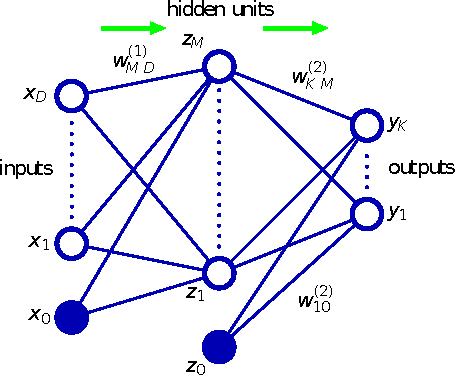
\includegraphics[width=0.6\textwidth]{Figures/deep-feedforward-network.pdf}
\decoRule
\caption[Representación de una \textsl{Deep Feedforward Network}]{Representación de una \textsl{Deep Feedforward Network}. Tomado de \cite{bishop-pattern-recognition}.}
\label{fig:deep-feedforward-network}
\end{figure}

Aunque esta es una representación simplificada de este tipo de redes, este libro no tratara de profundizar en los detalles técnicos al ser estos muy amplios (véase \cite{deeplearning} y \cite{bishop-pattern-recognition}).

\subsection{Redes neuronales recurrentes (\glsentrylong{rnn})}
\todo[inline]{Expandir capitulo con contenido de pag 368 de Deep Learning}
La naturaleza recurrente de estas redes viene del hecho de representarse como redes donde su salida hace parte de la entrada a la siguiente iteración de la red, tal como se aprecia en la \figureref{fig:rnn-classic-simple}.

\begin{figure}[H]
  \centering
  % \missingfigure{Hacer la arquitectura en yEd}
  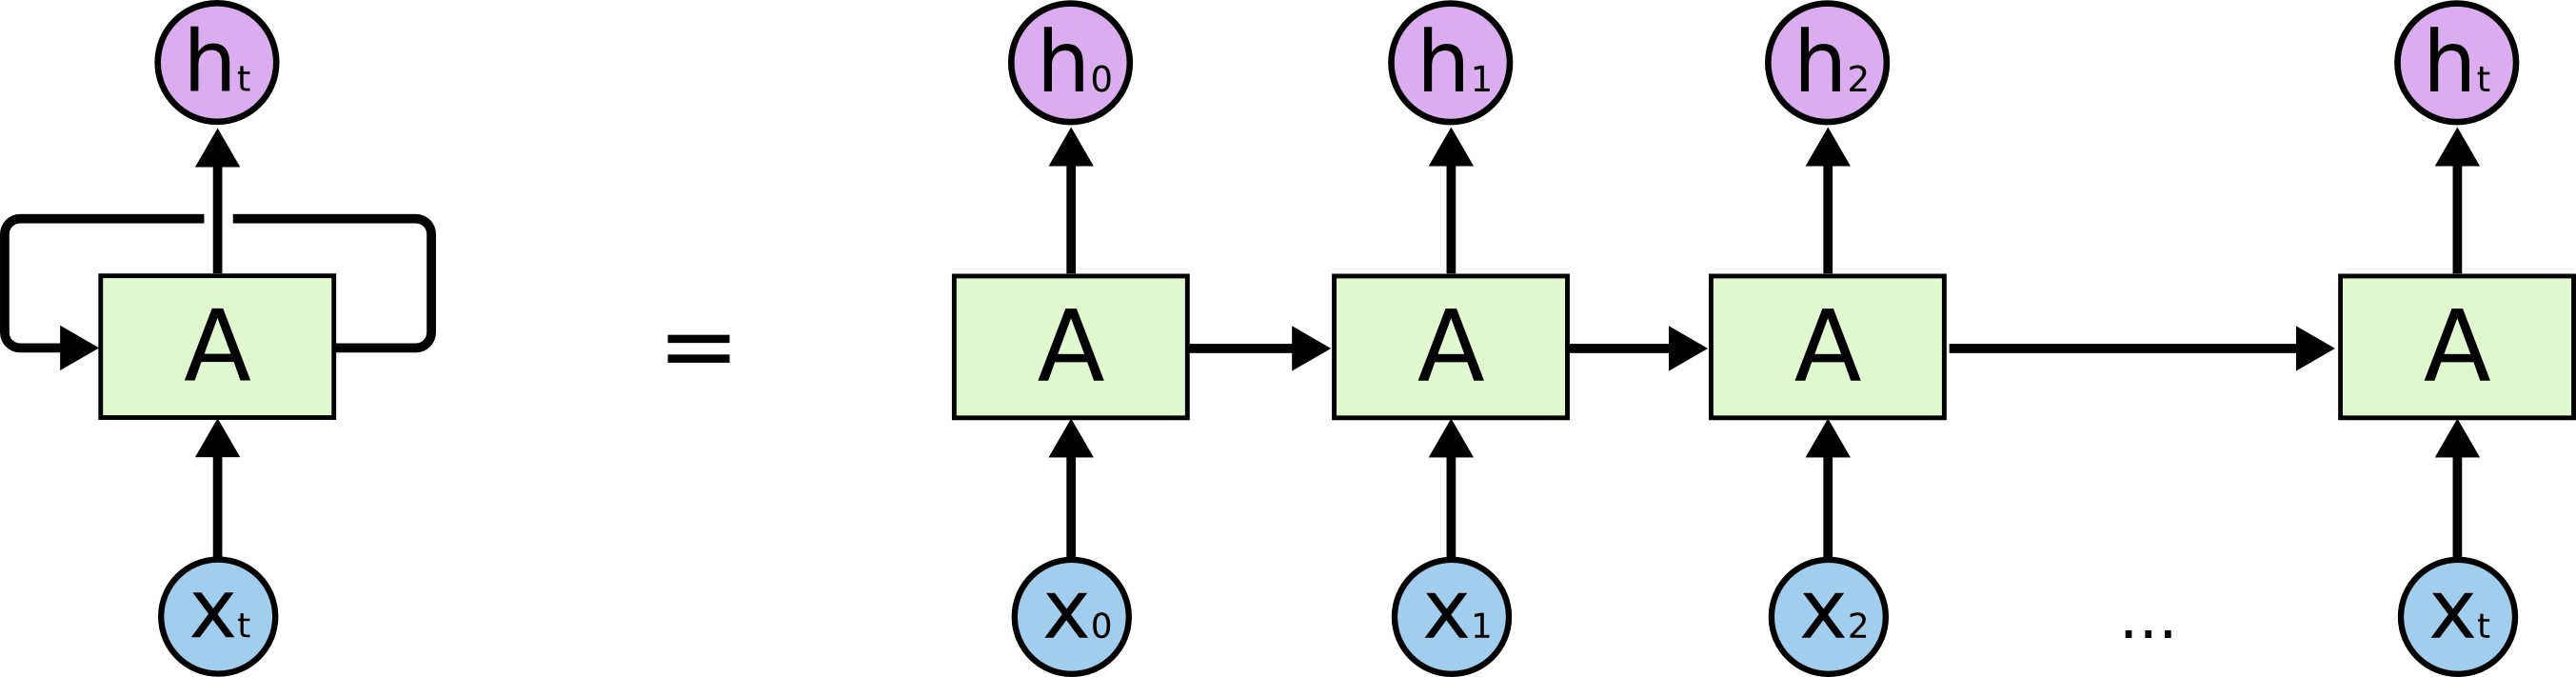
\includegraphics[width=0.8\textwidth]{Figures/RNN-unrolled.png}
\decoRule
\caption[Red \glsentrytext{rnn} simplificada]{Red \glsentrytext{rnn} simplificada. Tomado de \cite{understanding-lstm}.}
\label{fig:rnn-classic-simple}
\end{figure}

Este tipo de redes tiene la característica de recordar salidas y entradas pasadas de datos, de forma que decisiones futuras respecto a una clasificación pueden tener una mejor forma de basarse\todo{ajustar la redaccion de esta frase}. Las redes neuronales (\glspl{ann}) típicamente no pueden hacer estas operaciones ya que no tienen incorporada la habilidad de recordar entradas y salidas pasadas, sino que se realiza un entrenamiento con información de entrada y de salida que se conoce con anticipación, de forma que su salida solo se concentra en su entrada inmediata de datos.

Por este motivo, las \glspl{rnn} poseen una gran ventaja en situaciones puntuales, tales como el caso expuesto al inicio de esta sección (\gls{namedent}), sin embargo, el modelo clásico de \gls{rnn} es como la arquitectura presentada en la \figureref{fig:rnn-classic}, esta no provee resultados significativos debido a limitantes respecto al nivel de recordación que tienen originalmente.\todo[inline]{creo que hay que ajustar este parrafo porque primero se dice que las RNN son muy buenas y traen grandes ventajas por su capacidad de recordación y luego se termina diciendo que no provee resultados significativos. Por favor ajustar para que sea mas objetivo y no se vea la contradicción}

\subsection{Redes neuronales recurrentes bidireccionales (\glsentrylong{birnn})}
\todo[inline]{Por hacer, con pag 383 Deep Learning}

% ================================================================
% ================================================================

\section{Clasificación} \label{subsec:clasification}
Clasificación es la tarea de asignarle una de varias categorías predefinidas a objetos, y es una tarea que tiene una variedad extensa de aplicaciones. Ejemplos de esto se encuentran la detección de correos no deseados en mensajes de e--mails basándose del encabezado o el cuerpo del mensaje, categorización de células benignas de malignas basándose en los resultados de escaneados MRI o incluso la clasificación de galaxias basado en su forma.

Definido formalmente, clasificación es la tarea de aprender una función objetivo $f$ que mapea cada conjunto de atributos $x$ a una clase predefinida de etiquetas $y$.

La función objetivo también se define informalmente como un \emph{modelo de clasificación}.

% ================================================================

\subsection{Sistemas Basados en Conocimiento (\glsentrylong{kbs})} \label{sec:KBS}
\todo[inline]{Explicar bien en que consiste la base de conocimiento y el motor de inferencia}
Según \cite{sajja2010knowledge}, los \gls{kbs} son uno de los mayores miembros de la familia de \gls{ai}. El \gls{kbs} consiste de una \gls{knowledgebase} y un programa de búsqueda llamado \gls{inferenceengine} representado en la \figureref{fig:kbs-arch}. La \gls{knowledgebase} puede ser usado como un repositorio de conocimiento de varias formas.

Existen 5 tipos de \gls{kbs}\todo{Explicar brevemente cada uno de los 5 tipos}, donde uno de ellos es conocido como \gls{expertsystems}, usados como \gls{rulebasedsys}, donde su \gls{knowledgebase} esta dado como reglas y el \gls{inferenceengine} esta dado por algo llamado \gls{workingmemory}, que representa los hechos que se conocen inicialmente del sistema junto con los nuevos hechos que se van dando como inferencia de las reglas.

\begin{figure}[H]
\centering
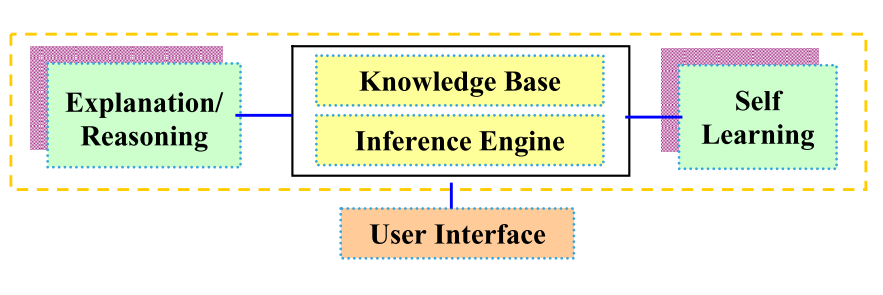
\includegraphics[scale=0.4]{Figures/kbs-architecture.png}
\decoRule
\caption[Arquitectura \glsentrytext{kbs}]{Arquitectura \glsentrytext{kbs}. Tomado de \cite{sajja2010knowledge} \todo[inline]{Explicar esta figura: Que significa explanation/reasoning, self-learning y User Interface}}
\label{fig:kbs-arch}
\end{figure}

Estas reglas pueden resumirse como una colección de condicionales de la forma \textbf{IF/ELSE} que se componen de un \emph{antecedente} y un \emph{consecuente}.

Existen dos tipos de \gls{rulebasedsys}, definidos como \gls{deductivesys} y \gls{reactivesys}, donde el \gls{deductivesys} tiene como objetivo realizar una conclusión en base a los hechos iniciales en la \gls{workingmemory}, por el otro lado se tienen los \gls{reactivesys}, los cuales de igual manera a los \gls{deductivesys}, toman los hechos de la \gls{workingmemory} y realizan sea una acción interactiva con su entorno o bien una modificación de los hechos que se encuentran en la \gls{workingmemory} tal como la adición o eliminación de hechos. Tómese el ejemplo de la \equationref{eq:rbs-example} tomada de \cite{Mendel}, donde \emph{x} es la temperatura y \emph{AC} es aire acondicionado.

\begin{equation} \label{eq:rbs-example}
  \left\{ \begin{array}{ll}
            \text{IF x es moderado,} & \text{THEN y = ajustar AC a bajo} \\
            \text{IF x es alto,}     & \text{THEN y = ajustar AC a moderado a alto} \\
            \text{IF x es muy alto,} & \text{THEN y = ajustar AC a alto} 
          \end{array} \right.
\end{equation}

\subsubsection{Tipos de \glsentrylong{kbs}} \label{ch:kbs-types}
\todo[inline]{Pendiente}

\subsubsection{\glsentrylong{rulebasedsys}} \label{ch:kbs-rule-based-system}
\todo[inline]{Por acomodar y expandir}

% ================================================================

\subsection{Maquina de soporte vectorial (\glsentrylong{svm})} \label{sec:SVM}
\gls{svm} es una técnica de clasificación que tiene sus raíces en la teoría de aprendizaje estadístico que ha mostrado resultados empíricos prometedores en muchas aplicaciones practicas, desde reconocimiento de dígitos escritos a mano a categorización de texto. \gls{svm} también funciona muy bien con datos de alta dimensionalidad. Otro aspecto destacable de esta aproximación es que representa la frontera de decisión usando un subconjunto de las muestras de entrenamiento, conocidos como los \emph{support vectors}.

\subsubsection{Maximum Margin Hyperplanes}
Se puede entender a los \gls{mmh} como hiper-planos que ayudan a separar datos en un hiper-espacio y que poseen un margen de decisión entre los datos, como ejemplo tómese la \figureref{fig:svm-hyperplanes}, donde el hiper-plano $B_1$ tiene un margen de decisión mas grande que el hiper-plano $B_2$.

\begin{figure}[H]
   \centering
   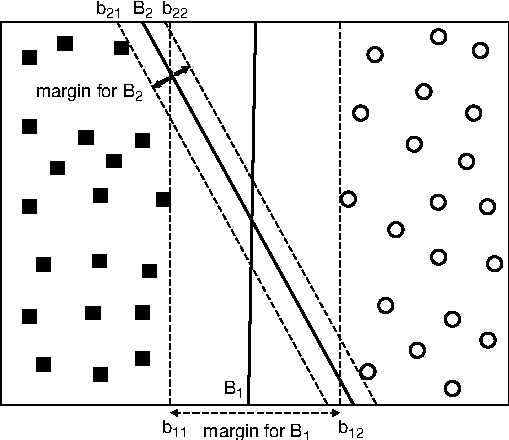
\includegraphics[width=0.7\textwidth]{Figures/svm-hyperplanes.pdf}
   \decoRule
   \caption[\glsentryname{mmh}]{\glsentryname{mmh}. Tomado de \cite{tan2005introduction}}
   \label{fig:svm-hyperplanes}
\end{figure}

Finalmente, el objetivo final de los \gls{svm} es la búsqueda de un hiper-plano con el mayor margen de decisión. Existen dos tipos de \gls{svm}, el lineal y el no--lineal. El lineal realiza la separación de los datos con su hiper-plano a partir de los datos de entrada en su espacio vectorial original, mientras que el no--lineal consta de realizar una transformación de los espacios de los datos de entrada a uno en que sea linealmente separable (véase como ejemplo la \figureref{fig:svm-nonlinear-transforms}), sin embargo al realizar la transformación, el algoritmo de \gls{svm} se ve afectado por la dimensionalidad de la entrada, por lo que existe lo que se conoce como la función \emph{kernel} para remediarlo.

Estas limitantes de dimensionalidad ocurren por un problema conocido como la \textbf{maldición de dimensionalidad} (o \textsl{curse of dimensionality} en inglés), y se manifiesta cuando el numero de dimensiones en los datos es alta. Particularmente se debe tener muy presente que el numero de configuraciones distintas posibles de un conjunto de variables crezcan de manera exponencial a medida que el numero de variables aumenta. Este caso ocurre con los \glspl{svm} cuando se vuelve necesaria la conversión de espacios vectoriales.

\begin{figure}[H]
   \centering
   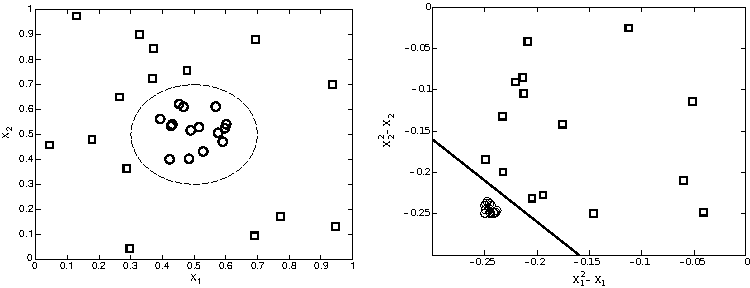
\includegraphics[width=0.95\textwidth]{Figures/svm-nonlinear-transform.pdf}
   \decoRule
   \caption[Transformación de espacios en \glsentrylong{svm}]{Transformación de espacios en \glsentrylong{svm}. Tomado de \cite{tan2005introduction}}
   \label{fig:svm-nonlinear-transforms}
\end{figure}

\subsubsection{Función Kernel}
La función polinomial de similaridad, $K$, la cual es calculada en el espacio original de los datos de entrada, se le conoce como la \textbf{función Kernel}. En principio se asegura que la función kernel puede ser expresada siempre como el producto punto entre dos vectores de entrada en algún espacio de alta dimensionalidad, la función de kernel también tiene la particularidad de que el computo de los productos punto con la función toman considerablemente menos tiempo que realizar la transformación de espacios, dejando de lado la transformación, acelerando la tarea de clasificación.

% ================================================================

\subsection{Clasificadores Bayesianos} \label{sec:bayes}
En muchas aplicaciones practicas las relaciones entre un conjunto de atributos y una serie de clases son inciertas. Es decir, la clase a la que pertenece un atributo de prueba no es posible predecirlo con completa certeza incluso si el atributo es identico a alguno de entrenamiento. Esta situacion se puede presentar por ruido en el conjunto de datos o bien por factores ajenos que afectan la clasificacion pero que no fueron incluidos en el analisis del problema.

Es por esto que es necesario establecer un modelo que utilice relaciones probabilisticas entre sus atributos y sus clases. Debido a esto es util tener presente el \textbf{teorema de Bayes}, un principio estadistico que combina conocimiento previo con nueva evidencia recolectada a partir de los datos.

\subsubsection{Teorema de Bayes} \label{subsec:bayestheo}
El teorema de Bayes dice que para un par de variables aleatorias $\rx$ e $\ry$, donde $P(\rx=x \mid \ry=y)$ es la probabilidad de que la variable $\rx$ tome el valor $x$ dado que el valor de la variable $\ry$ es $y$. Se tiene entonces la \equationref{eq:bayestheo}.
\begin{equation} \label{eq:bayestheo}
  P(\ry \mid \rx) = \frac{P(\rx \mid \ry) P(\ry)}{P(\rx)}
\end{equation}

\paragraph{Usando el teorema de Bayes para clasificación}
Para denotar el problema de clasificación desde una perspectiva estadística, definimos a $\sX$ y $\sC$ como el conjunto de atributos y el conjunto de etiquetas de clase. Si las etiquetas de clase y los atributos tienen una relación incierta, entonces se puede tomar a $\rx \in \sX$ y $\rc \in \sC$ como variables aleatorias y establecemos a $P(\rc \mid \rx)$ como su relación probabilística de que $\rx$ pertenece a la clase $\rc$.

Durante la fase de entrenamiento, es necesario aprender las probabilidades de $P(\rc \mid \rx)$ basándose únicamente en los datos recolectados de los datos de entrenamiento.

Luego de entrenar el clasificador, la forma en que podemos determinar una clase concreta $c \in \sC$ para un atributo concreto $x \in \sX$ es por medio de encontrar la combinación que nos de una mayor probabilidad de nuestro modelo, dándonos una estimación de la clase con $\hat{c}$, tal como se muestra en la \equationref{eq:bayes-clasification-argmax}.

\begin{equation} \label{eq:bayes-clasification-argmax}
  \hat{c} = \argmax_{c\in\sC} P(\rc = c \mid \rx = x)
\end{equation}

\subsubsection{Clasificador Na\"{\i}ve Bayes} \label{subsec:naivebayes}
Un clasificador de Na\"{\i}ve Bayes estima la probabilidad condicional de las clases por medio de suponer que los atributos son condicionalmente independientes \mbox{(e.g. $x_i \bot x_j \mid \rc, \forall i, j$)}, dado la etiqueta de clasificación $c$. La suposición de independencia condicional se puede dar por la \equationref{eq:bayes-conditional-independence}.

\begin{equation} \label{eq:bayes-conditional-independence}
  P(x_i \mid \rc, x_j) = P(x_i \mid \rc), \, i \neq j, \, \forall i, j \in \{1, \ldots, d\}
\end{equation}

Donde cada conjunto de atributos $\sX=\{ x_1, \ldots, x_d \}$ consiste de $d$ atributos.
\paragraph{Como funciona el clasificador Na\"{\i}ve Bayes}
Con la suposición de independencia condicional, en vez de computar la probabilidad condicional de clases para cada combinación de $\sX$, solo se debe realizar para establecer la probabilidad condicional de cada $x_i$, dado $\rc$.

Para clasificar un dato de prueba, el clasificador computa la probabilidad posterior para cada clase $\ry$ como se muestra en la \equationref{eq:bayes-classifier}.

\begin{equation} \label{eq:bayes-classifier}
  P(\rc\mid \sX) = \frac{P(\rc) \prod_{i=1}^{d}P(x_i\mid\rc)}{P(\sX)} \Rightarrow P(\rc) \prod_{i=1}^{d}P(x_i\mid\rc)
\end{equation}

Puede ignorarse $P(\sX)$ debido a que es un termino constante. Para esto se realiza una normalización de forma que $\sum_{\forall \rc \in \sC} P(\rc\mid \sX) = 1$.

% ================================================================

\subsection{$k$ vecinos mas cercanos (\glsentrylong{knn})}
El algoritmo de los $k$ vecinos mas cercanos (o \gls{knn} en inglés) es un algoritmo no-parámetrico que tiene como objetivo encontrar los $k$ elementos mas cercanos en un conjunto de datos de entrenamiento $\train$ a una entrada $\vx$, cuenta cuantos miembros de cada clase están en el conjunto (cada elemento del conjunto ya tiene una clase definida), y retorna una fracción empírica como estimado. Formalmente como
\begin{equation} \label{eq:prob-knn}
  p(y = c \mid \rvx, \train, k) = \frac{1}{k} \sum_{i \in N_k(\rvx, \train)} [y_i = c]
\end{equation}

donde $N_k(\vx, \train)$ son los índices de los $k$ vecinos mas cercanos a $\rvx$ en $\train$ y $[\mathrm{condition}]$ es el \textbf{indicador}, que toma el valor de $1$ cuando la condición es verdadera y $0$ de lo contrario.

Dada la probabilidad de pertenencia de una clase con la \equationref{eq:prob-knn} se puede entonces estimar cual es la clase a la que pertenece un punto $\vx$ por medio de estimar la clase que maximice la probabilidad que se estimo anteriormente como
\begin{equation}
  \hat{y}(\vx) = \argmax_{c} p(y = c \mid \rvx = \vx, \train)
\end{equation}

\begin{figure}[H]
  \centering
  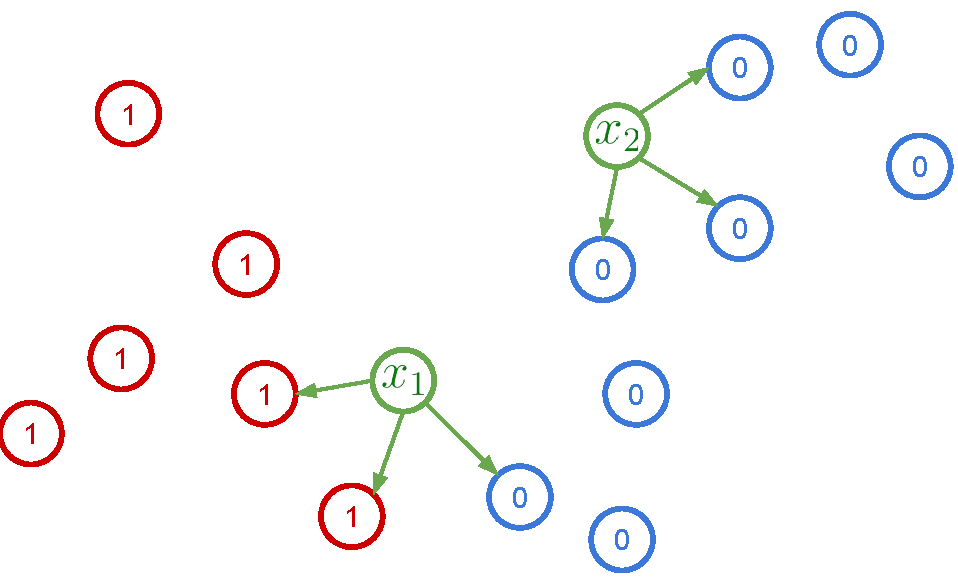
\includegraphics[width=0.60\textwidth]{Figures/knn-example.pdf}
  \decoRule
  \caption[Ejemplo de algoritmo de \textsl{\glsentrylong{knn}}]{Ejemplo de algoritmo de \textsl{\glsentrylong{knn}} en 2-D para $k = 3$, los 3 vecinos mas cercanos a $\vx_1$ tienen etiquetas de $1, 1, 0$, así que se predice la probabilidad $p(p = 1 \mid \rvx = \vx_1, \train, k=3) = 2/3$, Los 3 vecinos mas próximos a $\vx_2$ tienen etiquetas de $0, 0, 0$, por lo que la probabilidad de predicción es $p(y=1 \mid \rvx = \vx_2, \train, k=3) = 0/3$. Basado de \cite{murphymachinel}.}
  \label{fig:knn-example}
\end{figure}

Tómese como ejemplo la \figureref{fig:knn-comparisons}, en donde se muestra un conjunto de entrenamiento $\train$, las distribuciones de probabilidad dadas para las clases 1 y 2, como también una gráfica que muestra como se clasifica una muestra dependiendo de su ubicación en el espacio.

\begin{figure}[H]
   \centering
   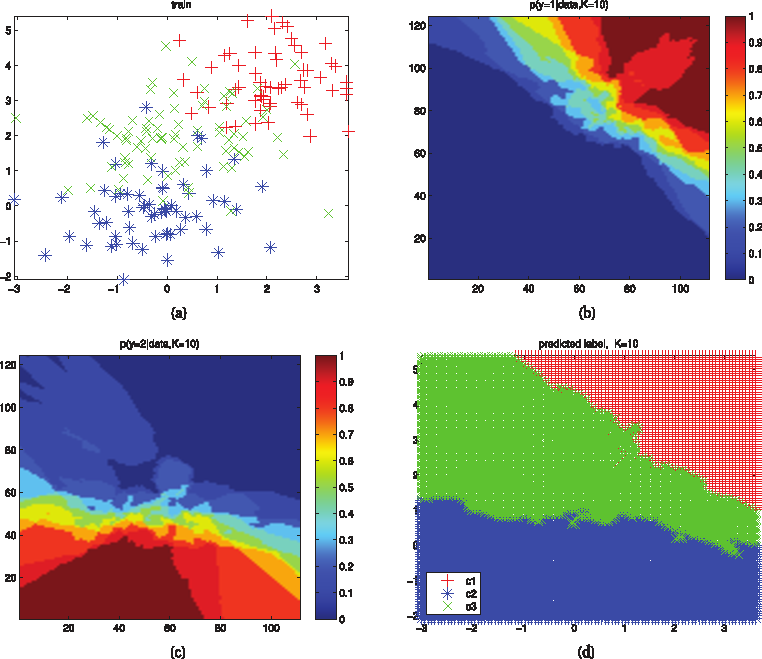
\includegraphics[width=0.9\textwidth]{Figures/knn-comparisons.pdf}
   \decoRule
   \caption[Comparaciones de \textsl{\glsentrylong{knn}}]{Comparaciones de \textsl{\glsentrylong{knn}}, $k=10, n=2$. (a)~Conjunto de entrenamiento $\train$, (b)~Dibujo de $p(y=1 \mid \rvx, \train)$, (c)~Dibujo de $p(y=2 \mid \rvx, \train)$, (d)~Dibujo de $\hat{y}(\rvx) = \argmax_{c} p(y=c \mid \rvx, \train)$. Tomado de \cite{murphymachinel}.}
   \label{fig:knn-comparisons}
\end{figure}

% ================================================================

\subsection{Sistemas de Detección de Anomalías (\glsentrylong{anomalydetectionsys})}
Existen diferentes aproximaciones para los sistemas de anomalías, sin embargo una similitud entre todos estos sistemas es que se intenta realiza una \emph{detección de desviaciones}, y su tarea es detectar los datos \emph{atípicos} en un sistema \cite{tan2005introduction}.

Uno de los que se pueden encontrar en la literatura son los sistemas de detección de anomalías basados en realizar un estimado probabilístico con alguna distribución de probabilidad de donde para una serie de características $m$ se trata de estimar una distribución gaussiana $\rmX \sim \mathcal{N}(\mu, \sigma^2)$ que tiene media $\mu$ y varianza $\sigma^2$ por cada característica, por lo que existirán $m$ diferentes distribuciones .

Para estimar cada una las medias y variaciones de cada característica $j$, $\mu$ se estima con la \equationref{eq:anomaly-mu} y $\sigma^2$ se estima con la \equationref{eq:anomaly-sigma}.

\begin{equation} \label{eq:anomaly-mu}
  \mu_j = \frac{1}{m} \sum_{i=1}^{m} x_j^{(i)}
\end{equation}

\begin{equation} \label{eq:anomaly-sigma}
  \sigma_j^2 = \frac{1}{m} \sum_{i=1}^{m} (x_j^{(i)} - \mu_j)^2
\end{equation}

De donde para calcular la probabilidad de que una muestra se trata de una anomalía se calcula la probabilidad $p(x)$, luego de que fueron estimadas las distribuciones de cada característica del conjunto de entrenamiento, por lo que se define un $\epsilon$ de manera heurística, de forma que se determina que una muestra anómala si $p(x) < \epsilon$, la \equationref{eq:anomaly-prob} representa cual es la probabilidad de una muestra $x$ con una distribución gaussiana.

\begin{equation} \label{eq:anomaly-prob}
  p(x) = \prod_{j=1}^{n}p(x_j, \mu_j, \sigma_j^2) = \prod_{j=1}^{n} \frac{1}{\sqrt{2\pi}\sigma_j} \exp\Bigg( - \frac{(x_j-\mu_j)^2}{2\sigma_j^2}\Bigg)
\end{equation}

Si el modelo esta dando como resultado muchos falsos positivos, lo que se debe hacer es reducir $\sigma$.

Este método de sistemas de detección de anomalía también es brevemente tratada en \cite{osint} con una representación de hiper-planos, que es equivalente con este descrito.

% ================================================================
% ================================================================

\section{Clustering} \label{subsec:clustering}
El análisis de clusters agrupa objetos de datos basándose únicamente en la información encontrada en los datos que describen los objetos y sus relaciones. El objetivo es que objetos dentro de un grupo sean similares (o relacionados) el uno al otro, y que sean diferentes (o sin relación) a objetos en otros grupos. Entre mayor sea la similitud dentro de un grupo y entre mayor sea la diferencia entre grupos, sera mejor o mas distintivo el clustering.

Los métodos de clustering se hacen referencia comúnmente en \gls{machinel} como métodos no--supervisados. Un método de estos es el algoritmo de $k$-means y el de mapas autoorganizados que se describen a continuación.

% ================================================================

\subsection{Algoritmo de $k$-means}
El algoritmo de $k$-means consiste en intentar encontrar $k$ subconjuntos de datos disyuntos tales que la diferencia entre las características de los miembros sea lo mas disimilares. Esto lo logra a partir de definir $k$ \textit{centroides} inicializados aleatoriamente sobre el conjunto de datos. El valor $k$ es puesto de antemano a la ejecución del algoritmo por el usuario. Cada elemento en el conjunto de datos se es asignado el $i$-ésimo centroide mas cercano. Luego se recalculan los centroides a partir de ponderar todos los puntos que fueron asignados a cada centroide. Este proceso se repite hasta que el cambio de posición del centroide sea marginal. Tómese de referencia el Algoritmo~\ref{algo:k-means} y la \figureref{fig:k-means-iterations} donde se pueden ver las iteraciones del algoritmo.

\IncMargin{1em}
\begin{algorithm}[H]
  \Entrada{Conjunto de datos $\mX \in \R^{n \times m}$ y valor de $k$}
  \Salida{Centroides $\{ \vmu^{(1)}, \ldots, \vmu^{(k)} \}$}
  
  Inicialización aleatoria de los $k$ puntos $\{ \vmu^{(1)}, \ldots, \vmu^{(k)} \} \,;\, \forall j, \vmu^{(j)} \in \R^{n}$\;
  Define vector $\vh \in \{1, \ldots, k\}^{m}$ representando la asignación de centroides a cada punto de $\mX$\;
  \Repetir{Ningún centroide cambia (e.g. $\norm{\vmu_t^{(i)} - \vmu_{t-1}^{(i)}} \approx 0, \forall i$)}{
    \ParaTodo{$\vx_i \in \mX$}{
      $\vh_i \leftarrow \argmin_{j} \norm{\vx_i - \vmu^{(j)}}$\;
    }

    \ParaTodo{$\vmu^{(j)} \in \{ \vmu^{(1)}, \ldots, \vmu^{(k)} \}$}{
      $sz \leftarrow \sum_{i} [ \vh_i = j ]$\;
      $\vmu^{(j)} \leftarrow \frac{1}{sz} \sum_{i} \vx_i \cdot [ \vh_i = j ]$\;
    }
  }
  
  \caption{$k$-means simplificado.}
  \label{algo:k-means}
\end{algorithm}
\DecMargin{1em}

Es útil mencionar que en este algoritmo puede valer la pena ejecutarlo mas de una vez. La inicialización aleatoria de los $k$ centroides puede tener un inicio mas beneficioso para la clusterización de manera que este mejor distribuida una vez se alcanza un estado de convergencia.

\begin{figure}[H]
  \centering
  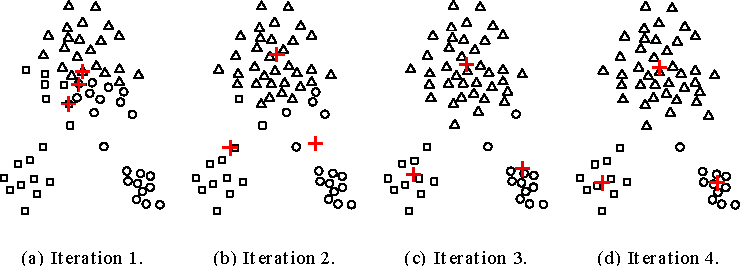
\includegraphics[width=0.9\textwidth]{Figures/k-mean-iteration.pdf}
  \decoRule
  \caption[Iteraciones del algoritmo de $k$-means]{Iteraciones del algoritmo de $k$-means, $n = 2, k = 3$, centroides marcados en rojo. Tomado de \cite{tan2005introduction}.}
  \label{fig:k-means-iterations}
\end{figure}

% ================================================================

\subsection{Mapa autoorganizado (\glsentrylong{som})} \label{subsec:SOM}
Las \glspl{som} son otra arquitectura de \glspl{ann} muy populares, sin embargo a diferencia de la arquitectura de las redes \gls{mlp}, esta consta de una sola capa de neuronas, y no tiene un propósito de predicción, por lo que no es necesario aproximar ninguna función $f$ a una salida $\vy$ definida por un conjunto de entrenamiento.

El objetivo principal de los \glspl{som} es de transformar una patrón de entrada $m$--dimensional en un mapa discreto uni-- o bi--dimensional, donde sus principales características es que es un algoritmo que se basa en \gls{unsupervisedl}, es \gls{feedforward}, tiene una sola capa de neuronas donde su propósito es realizar \gls{clustering} y una reducción de dimensionalidad sobre los datos de una forma topológicamente ordenada.

Los \gls{som} tienen tres características distintivas:
\begin{itemize}
\item {\bf Competencia:} por cada patrón de entrada, las neuronas en la red competirán entre ellas para determinar un ganador.
\item {\bf Cooperación:} la neurona ganadora determina la ubicación espacial (vecinos) alrededor de donde otras vecinas también se verán estimuladas.
\item {\bf Adaptación:} la neurona ganadora como también sus vecinas tendrán sus pesos asociados actualizados, y se tiene que los vecinos entre mas cerca estén del ganador, mayor es el grado de adaptación.
\end{itemize}

El algoritmo de aprendizaje de \gls{som} parte de primero inicializar los pesos de las $o$ neuronas con pesos aleatorios pequeños de una distribución de probabilidad aleatoria o uniforme, donde cada vector de entrada se define como $\vx = [x_1, \ldots, x_m]^{\top} \in \R^{m}$ y la entrada general de $N$ patrones como $\mX^{m \times N}$, el vector de pesos de la neurona $i$ es $\vw_i = [w_{i1}, \ldots, w_{im}] \in \R^{1 \times m}$, con la matriz de pesos $\mW^{o \times m}$.

Para alcanzar el objetivo de \emph{competencia}, se realiza por cada patrón de entrada $\vx_i$ una comparación con cada uno de los pesos de las $o$ neuronas y se establece la de menor distancia $\norm{\vx}_p$ (típicamente la distancia Euclidiana o equivalentemente la norma $\normltwo$ e.g. $p = 2$), dejando un ganador $\mathrm{winner}$, tal como en la \equationref{eq:som-competition}.
\begin{equation} \label{eq:som-competition}
  \mathrm{winner} = \argmin_j \norm{\vx_i - \vw_j}_p ; j \in \{1, \ldots, o \}
\end{equation}

Luego de establecer la neurona ganadora, se realiza el paso para alcanzar la \emph{cooperación}, que consiste en que por medio de una función kernel $h$ (típicamente una una distribución gaussiana), que permite establecer un área de afectación de las otras neuronas según su ubicación física en el mapa, definidos como $\vr_{\mathrm{winner}}$ y $\vr_j$ que son la ubicación de la neurona ganadora y la neurona vecina $j$, en el cual el grado de afectación de la neurona vecina depende de la distancia $\normltwo$ de la que esta de la neurona ganadora, definido en la \equationref{eq:som-cooperation}.
\begin{equation} \label{eq:som-cooperation}
  h_{j, \mathrm{winner}}(t) = \exp\Bigg(\frac{- \norm{\vr_j - \vr_{\mathrm{winner}}}^2}{ 2 \sigma(t)^2}\Bigg)
\end{equation}

Parte importante del proceso de convergencia del \gls{som} es que a medida que avanzan las iteraciones $t$ del algoritmo el área de afectación se va reduciendo como parte del proceso de adaptación, por lo que definimos $\sigma(t) = \sigma_0 \exp(-t / \tau_1)$, donde $\tau_1$ es una constante heurística y $\sigma_0$ la dimensión del mapa \gls{som}.

Finalmente para alcanzar la \emph{adaptación} se realiza una actualización de los pesos de la matriz $\mW$ en base a la influencia de área $\sigma(t)$ y de una tasa de aprendizaje $\lr(t) = \lr_0 \exp(-t/ \tau_2)$, donde $\tau_2$ es otra constante heurística y $\lr_0$ es una constante de aprendizaje inicial, que debe ser $0 \le \lr_0 \le 1$, la actualización se describe por la \equationref{eq:som-adaptation} y el proceso puede ser visto gráficamente en la \figureref{fig:som-adap-proc}, tanto de forma uni-- como bi--dimensional.
\begin{equation} \label{eq:som-adaptation}
  \vw_j(t+1) = \vw_j(t) + \lr(t) h_{j, \mathrm{winner}}(t)\Big[\vx_i-\vw_j(t)\Big]
\end{equation}

\begin{figure}[H]
  \centering
  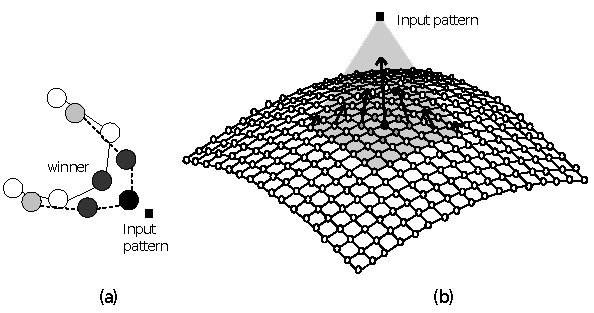
\includegraphics[width=0.75\textwidth]{Figures/som-adaptive-proc.pdf}
  \decoRule
  \caption[Proceso de adaptación de \glsentrytext{som}]{Proceso de adaptación de \glsentrytext{som}, (a) uni--dimensional, (b) bi--dimensional. Tomado de \cite{de2006fundamentals}}
  \label{fig:som-adap-proc}
\end{figure}

Luego de que el algoritmo de aprendizaje termina de realizar las iteraciones, la salida de este es la matriz de pesos $\mW$. En la \figureref{fig:som-impl-example} se puede apreciar una aproximación del algoritmo con un mapa uni--dimensional tratando de aproximar una función polar con ruido adicionado en un gráfico 2D. Adicionalmente pueden verse los efectos de \gls{underfitting} y \gls{overfitting} (véase el Apéndice \ref{appendix:keyconcepts}) con diferentes cantidades de neuronas en la \figureref{fig:som-impl-example-fitting}.

En la \figureref{fig:som-example} se puede ver una aplicación de los \gls{som}, en donde se realiza una clusterizacion de casos de homicidios donde los parámetros son características de los homicidios, según \cite{mena2003investigative} este resultado da una buena aproximación para sospechar de que estos son cometidos por personas distintas o si bien están siendo perpetrados por un mismo individuo o grupo.

\begin{figure}[H]
\centering
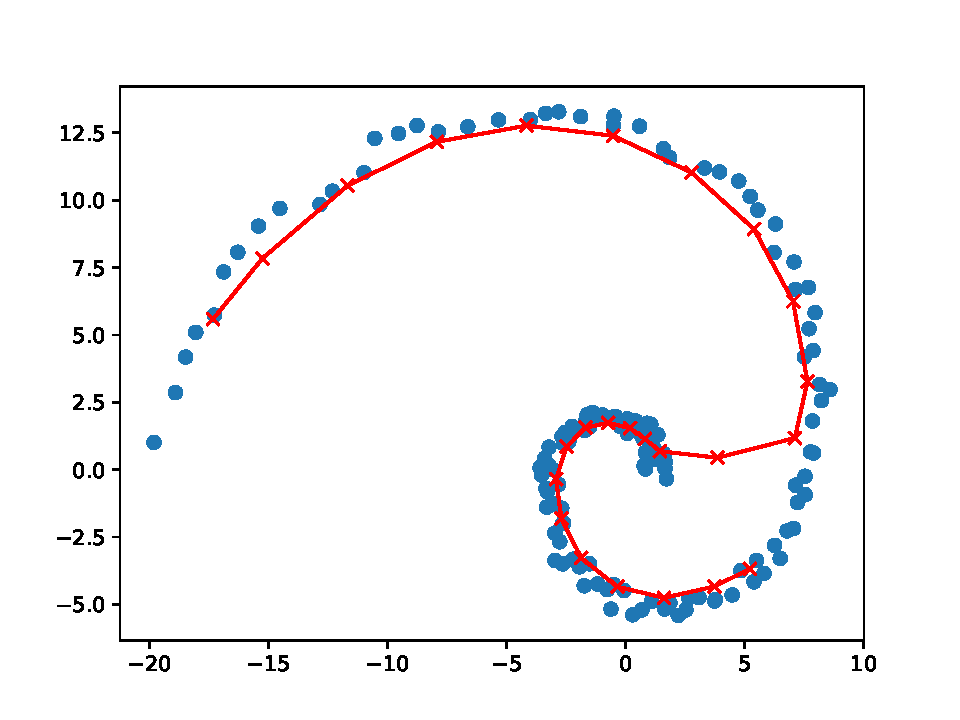
\includegraphics[width=\textwidth]{Figures/som-implementation-example25.pdf}
\decoRule
\caption[Ejemplo de salida de \glsentrytext{som} uni-dimensional]{Ejemplo de salida de \glsentrytext{som} uni-dimensional con 25 neuronas. Implementación propia.}
\label{fig:som-impl-example}
\end{figure}

\begin{figure}[H]
   \centering
   \begin{tabular}{ccc}
   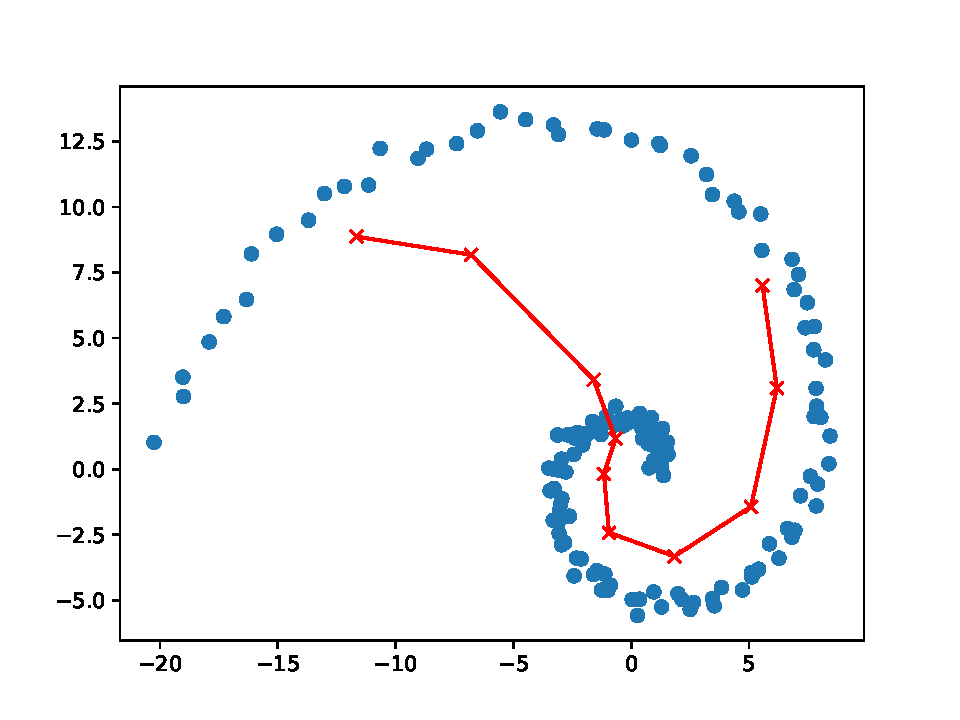
\includegraphics[width=0.32\textwidth]{Figures/som-implementation-example10.pdf} & %
   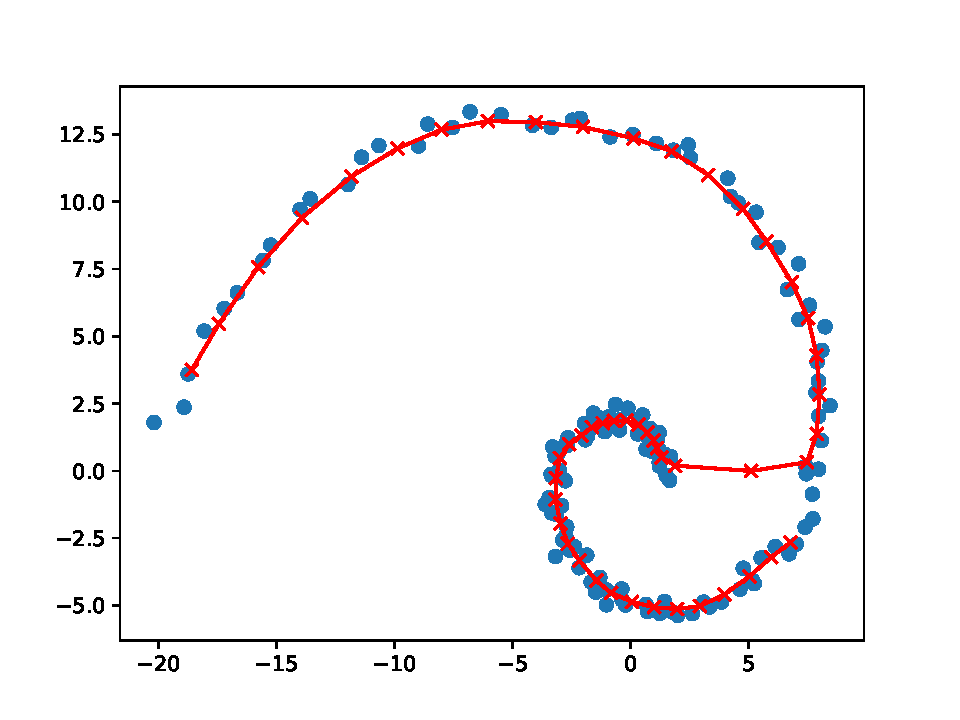
\includegraphics[width=0.32\textwidth]{Figures/som-implementation-example50.pdf} & %
   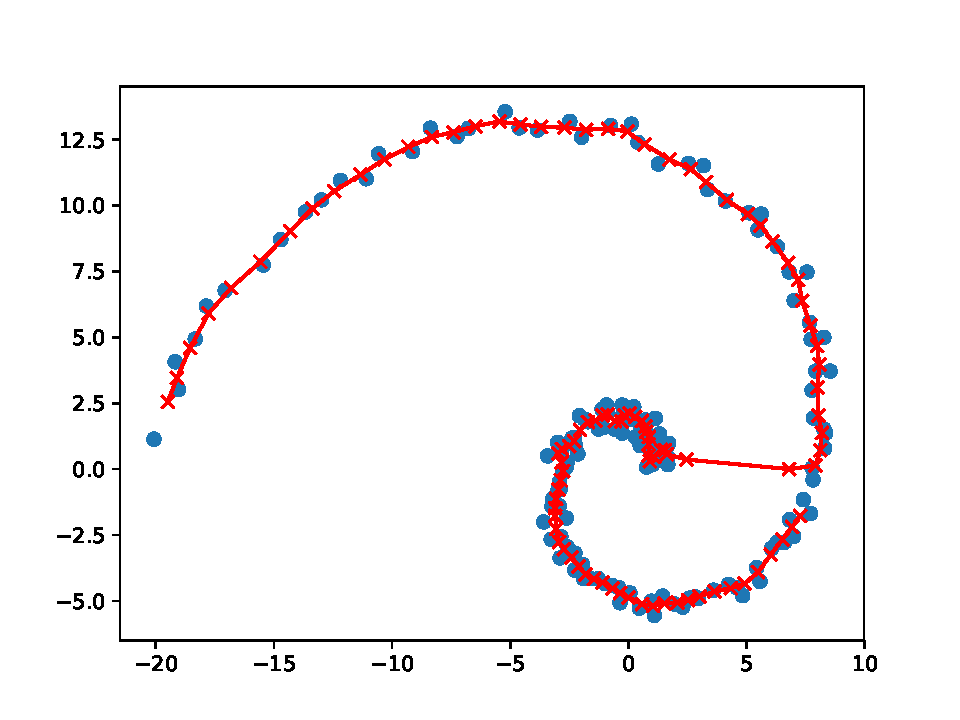
\includegraphics[width=0.32\textwidth]{Figures/som-implementation-example100.pdf} \\
     (a) & (b) & (c) \\ [1em]
   \end{tabular}
   \decoRule
   \caption[Comparación de salidas de \glsentrytext{som} uni-dimensional]{Comparación de salidas de \glsentrytext{som} uni-dimensional con (a) 10 neuronas (b) 50 neuronas y (c) 100 neuronas. Implementación propia.}
   \label{fig:som-impl-example-fitting}
\end{figure}

\begin{figure}[H]
\centering
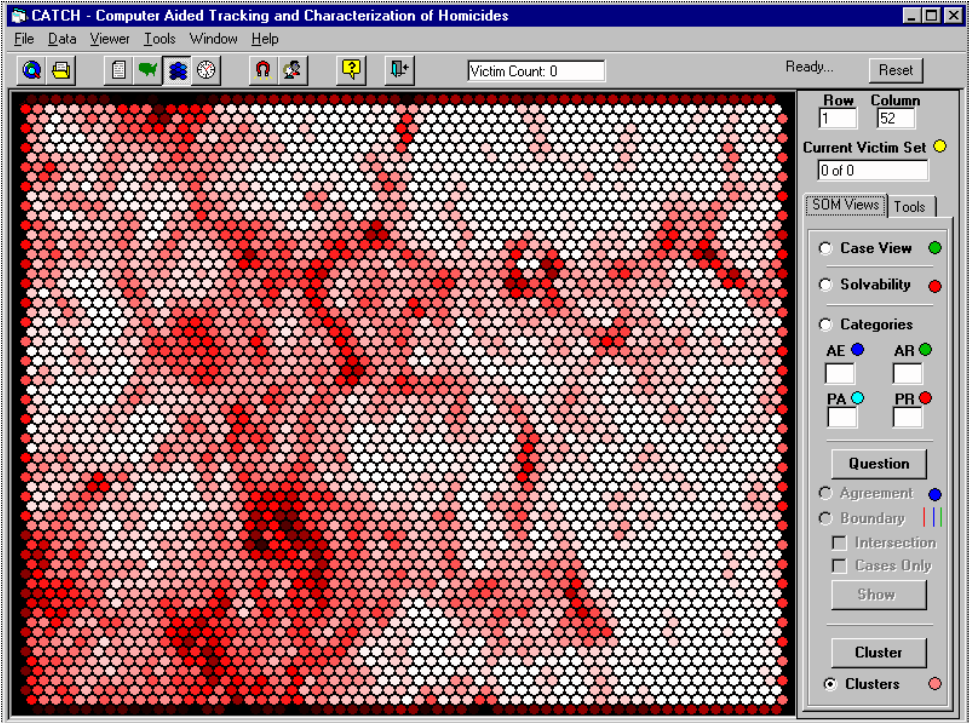
\includegraphics[width=\textwidth]{Figures/som-example.png}
\decoRule
\caption[Ejemplo de uso de \glsentrytext{som} en aplicaciones de perfilado]{Ejemplo de uso de \glsentrytext{som} en aplicaciones de perfilado. Tomado de \cite{mena2003investigative}}
\label{fig:som-example}
\end{figure}

% ================================================================
% ================================================================

\section{Procesamiento de lenguaje natural (\glsentrylong{nlp})}
% \todo[inline]{Por hacer, pagina 448 Deep Learning}
\todo[inline]{Por hacer, leer e incluir contenido de Speech and Language Processing \cite{jurafsky-martin}}
\todo[inline]{Por hacer, adaptar la seccion de propuesta para mencionar esta seccion}

El procesamiento de lenguaje natural (o \glsentrylong{nlp} en inglés), es el uso de lenguajes humanos, tales como el ingles, francés o español por un computador. Los programas de computador leen y emiten lenguajes especializados diseñados para un análisis eficiente y preciso por otros programas simples. Los lenguajes naturales son por lo general ambiguos y no poseen una definición formal. El procesamiento de lenguaje natural incluye aplicaciones tales como traducción de maquina, en el cual un aprendiz debe leer una sentencia en un lenguaje humano y emitir una sentencia equivalente en otro lenguaje humano. Muchas aplicaciones de \gls{nlp} se basan en modelos de lenguaje que definen una distribución de probabilidad sobre secuencias de palabras, caracteres o bytes en un lenguaje natural.

Para construir un modelo eficiente de lenguaje natural, debemos usar técnicas que son especializadas para el procesamiento de datos secuenciales. Por lo general nos interesa que el lenguaje natural sea representado como secuencias de palabras mas que otras posibles representaciones. Debido a que el numero total de palabras que existen es muy grande, modelos de lenguaje basados en palabras deben operar en espacios de muy alta dimensionalidad y discretamente dispersos.

\subsection{$n$-gramas}
Un \textbf{modelo de lenguaje} define una distribución de probabilidad sobre secuencias de tokens en un lenguaje natural. Dependiendo de como esta diseñado un modelo, un token puede ser una palabra, un carácter, o incluso un byte. Los tokens siempre son unidades discretas. Los primeros modelos de lenguaje exitosos se basaron en modelos de secuencias de tokens de tamaño fijo llamados $n$-gramas. Un $n$-grama es una secuencia de $n$ tokens.

Modelos que se basan en $n$-gramas definen la probabilidad condicional del $n$-ésimo token dados los $n-1$ tokens anteriores. El modelo usa productos de estas distribuciones condicionales para definir la distribución de probabilidad sobre secuencias mas largas:
\begin{equation}
  P(x_1, \ldots, x_\tau) = P(x_1, \ldots, x_{n-1}) \prod_{t = n}^{\tau} P(x_t \mid x_{t-n+1}, \ldots, x_{t-1})
\end{equation}

Esta descomposición se justifica con la regla de la cadena de probabilidad. La distribución de probabilidad sobre la secuencia inicial $P(x_1, \ldots, x_{n-1})$ puede ser modelado por un modelo diferente con un valor mas pequeño de $n$.

Usualmente cuando se entrenan modelos de $n$-gramas, se están entrenando tanto un modelo de $n$-grama como también un modelo de $(n-1)$-grama simultáneamente. Esto vuelve sencillo el calculo de
\begin{equation}
  P(x_t \mid x_{t-n+1}, \ldots, x_{t-1}) = \frac{P_n(x_{t-n+1}, \ldots, x_t)}{P_{n-1}(x_{t-n+1}, \ldots, x_{t-1})}
\end{equation}

por medio de solo tener al menos dos probabilidades calculadas (dos casos base).

Una limitante fundamental de estimación de máxima probabilidad sobre modelos de $n$-gramas es que $P_n$ como es estimado a partir del conteo del conjunto de entrenamiento es muy probable que sea igual a cero en muchos casos, trayendo consigo dos posibles problemas.

El primero es que cuando $P_{n-1}$ es diferente de cero pero $P_n$ es cero, la probabilidad logarítmica es $-\infty$, una mitigación a este problema que usan muchos modelos de $n$-gramas es realizar un \textbf{suavizado} sobre la distribución de probabilidad, haciendo que la probabilidad de tuplas nunca vistas aumente con la probabilidad de las tuplas mas vistas.

La segunda es que los modelos clásicos de $n$-gramas son particularmente vulnerables a la maldición de dimensionalidad (véase la \sectionref{sec:SVM}), debido a que existen $|\sV|^n$ posibles $n$-gramas, donde $|\sV|$ por lo general es grande.

\subsection{Modelos de lenguaje neural (\glsentrylong{nlm})}
\todo[inline]{Por hacer, pagina 451 Deep Learning}

\subsection{Etiquetado de \glsentrylong{pos}}
\todo[inline]{Por hacer, pagina 151 Speech and Language Processing \cite{jurafsky-martin}}

\subsection{\glsentrylong{hmm}}
\todo[inline]{Por hacer, pagina 464 Speech and Language Processing \cite{jurafsky-martin}}
\todo[inline]{Por hacer, pagina 312 y 603 Machine Learning \cite{murphymachinel}}